\ifx\PREAMBLE\UnDef
\documentclass{beamer}
\usepackage{tikz}
\usetikzlibrary{decorations.pathmorphing}
\usepackage[english]{babel}
% or whatever

\usepackage[latin1]{inputenc}
% or whatever
\usepackage{xifthen}
\usepackage{bsymb}
\usepackage{eventB}

\newBevt{evt}

\begin{document}
\else
\fi

\providecommand{\until}{\mathop{\mathcal{U}}}
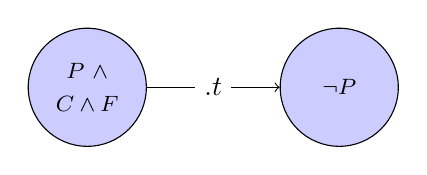
\begin{tikzpicture}[scale=0.8]
  \draw (2,0) node(s0)[circle, draw, fill=blue!20!white, inner sep =
  2pt, minimum width=1.5cm, align=center]{\footnotesize$P~\land$\\\footnotesize$C \land F$};
  \draw (6,0) node(s1)[circle, draw, fill=blue!20!white, inner sep =
  2pt, minimum width=1.5cm]{\footnotesize$\neg P$};
  \draw[->] (s0) --node[fill=white]{$\evt.t$} (s1);
\end{tikzpicture}

\ifx\PREAMBLE\UnDef
\end{document}
\else
\fi
